\documentclass[10pt]{beamer}

%%%
% PREAMBLE FOR THIS DOC 
%%%
%https://tex.stackexchange.com/questions/68821/is-it-possible-to-create-a-latex-preamble-header
\usepackage{/Users/miw267/Repos/latex_preamble/beamer_preamble}


\usepackage{bm}


%%%
% DOCUMENT
%%%

\begin{document}

%\maketitle

%% Title page frame
%\begin{frame}
%    \titlepage 
%\end{frame}



\title{10/28/2026: Big O, Big Omega, and Big Theta Notations}
\author{CSCI 246: Discrete Structures}
\date{Textbook reference: Ch 11.2, Epp}

\begin{frame}
    \titlepage 
\end{frame}


\begin{frame}
%\small
%\begin{mygreenbox}[title=Graded Quiz Pickup]
%Quizzes are in the front of the room, grouped into four bins (A-G, H-L, M-R, S-Z) by last name. The quizzes are upside down with your last name on the back. Come find yours before, during, or after class. Only turn the quiz over if it's yours.
%\end{mygreenbox} 
%\vfill 
%\begin{myredbox}[title=Friday's Problems Quiz]
%The problems quiz on Friday (04/02) will cover:
%\begin{itemize}
%\item Conditional Probability and Independence
%\item Random Variables
%\item Expectations	
%\end{itemize}
%
%\end{myredbox}
\vfill 
\begin{myyellowbox}[title=Today's Agenda]
\begin{itemize}
	\item Mini-lecture ($\approx$ 30 mins)
	\item Group exercises ($\approx$ 20 mins)
\end{itemize}
\end{myyellowbox}
\vfill 

\end{frame}


\begin{frame}
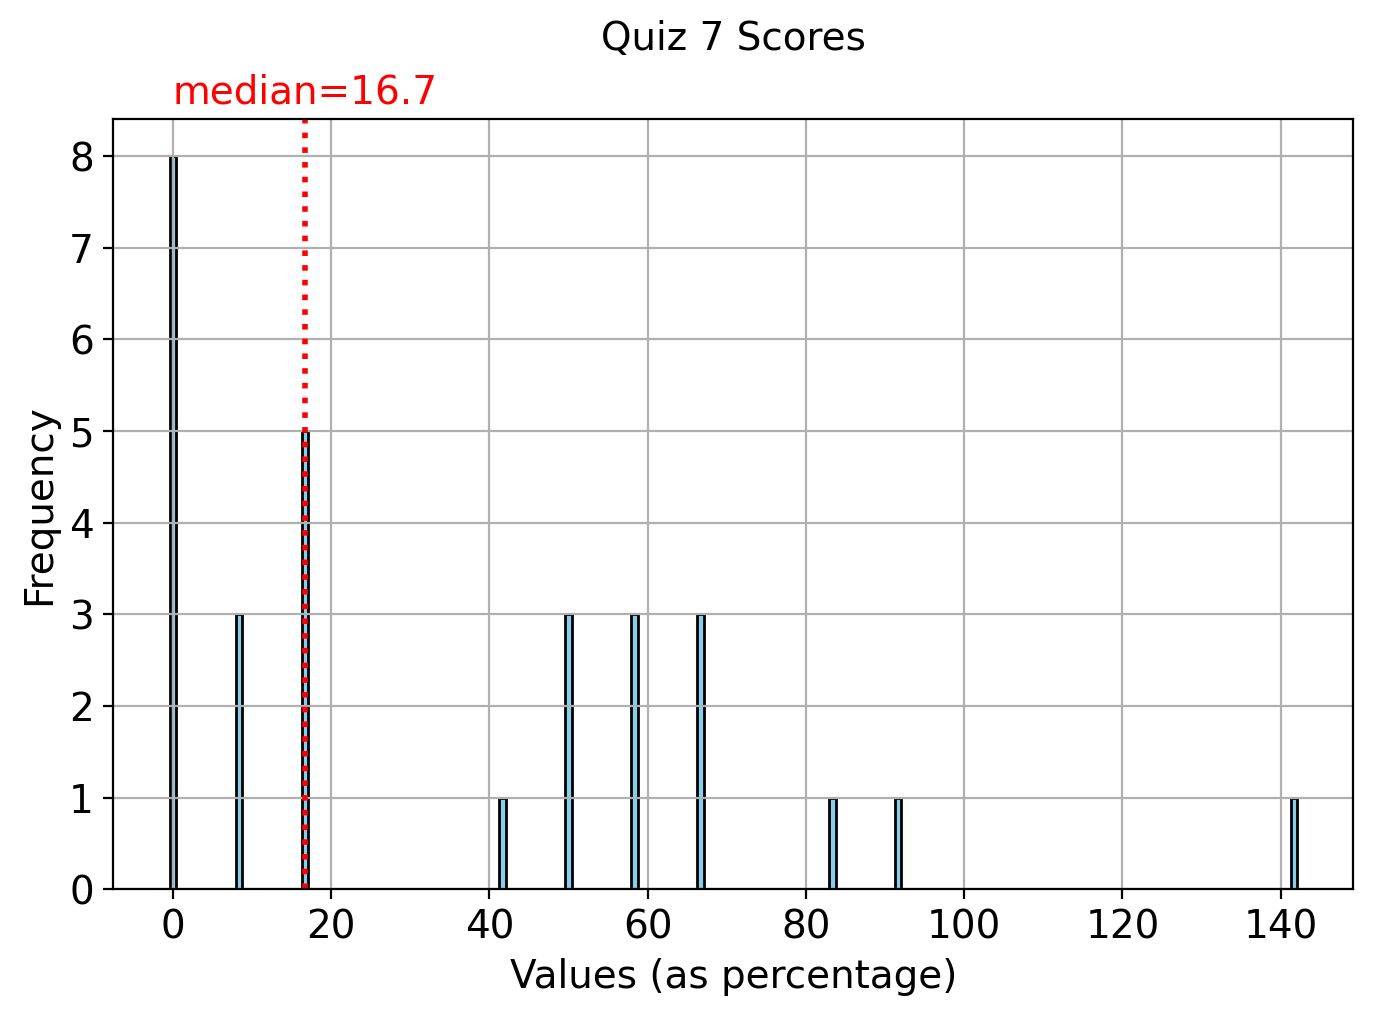
\includegraphics[width=.9\textwidth]{images/quiz_7_histogram.png}
	
\end{frame}


\begin{frame}{Study Guide For Quiz 8}
\footnotesize 

\colorbox{yellow!20}{\textbf{Group exercises.}} Know how to solve the group exercises from the course meetings on Induction (10/14) and Recurrence (10/16).


\vfill 

\colorbox{red!20}{\textbf{Readings.}}  \\
\vspace{.2cm}
Sec. 22 (Induction)
\begin{itemize}
\item Know how to use Theorem 22.2 / Proof Template 17 to prove Props. 22.3 and 22.5.
\item Understand the difference between Proof Template 17 and 18.
\end{itemize}
Sec. 23 (Recurrence)
\begin{itemize}
\item Know how to solve first-order recurrences from Props 23.1 and 23.3.  For example, see Example 23.2.
\item Know how to solve second-order recurrences from Theorems 23.5 and 23.9.  For example, see Example 23.6.
\item Know how to use Theorem 23.17 to find a polynomial expression to generate the first few terms of a sequence, as in Example 23.18.
\end{itemize}

\vfill 

\colorbox{green!20}{\textbf{Important Note.}} The max of your quiz 7 and quiz 8 scores will be used for both.
\end{frame}



\begin{frame}[standout]
Mini-lecture: \\
Big O, Big Omega, Big Theta Notations
\end{frame}

%\begin{frame}{Which would you rather have?}
%
%\begin{columns}[T]
%\begin{column}{0.47\textwidth}
%\begin{tcolorbox}[colback=blue!8, colframe=blue!60!black, halign=center, valign=center, height=3.2cm,
%  title=\textbf{Option A}, fonttitle=\large]
%\large \$1,000,000 on Nov 1
%\end{tcolorbox}
%\end{column}
%\begin{column}{0.47\textwidth}
%\begin{tcolorbox}[colback=orange!10, colframe=orange!80!black, halign=center, valign=center, height=3.2cm,
%  title=\textbf{Option B}, fonttitle=\large]
%\large \$1 on Nov 1, \\ doubled by the end of every day \\ for the month
%\end{tcolorbox}
%\end{column}
%\end{columns}
%
%\vfill
%
%\begin{columns}[T]
%\begin{column}{0.47\textwidth}
%\centering
%\onslide<2->{\textbf{Hopper} chooses Option A.}
%
%\vspace{0.4cm}
%\onslide<3->{On Nov 30: \\[2pt] {\Large \textbf{\$1,000,000}}}
%\end{column}
%\begin{column}{0.47\textwidth}
%\centering
%\onslide<2->{\textbf{Bob} chooses Option B.}
%
%\vspace{0.4cm}
%\onslide<3->{On Nov 30: \\[2pt] {\Large \alert{\textbf{\$1,073,741,824}}}}
%\end{column}
%\end{columns}
%
%\vfill
%\end{frame}

\begin{frame}{Which would you rather have?}

\begin{columns}[T]
\begin{column}{0.47\textwidth}
\begin{tcolorbox}[colback=blue!8, colframe=blue!60!black, halign=center, valign=center, height=2.4cm,
  title=\textbf{Option A}, fonttitle=\large]
\large \$1,000,000 on Nov 1
\end{tcolorbox}
\end{column}
\begin{column}{0.47\textwidth}
\begin{tcolorbox}[colback=orange!10, colframe=orange!80!black, halign=center, valign=center, height=2.4cm,
  title=\textbf{Option B}, fonttitle=\large]
\large \$1 on Nov 1, \\ doubled by the end of every day
\end{tcolorbox}
\end{column}
\end{columns}

\vfill

\begin{columns}[T]
\begin{column}{0.47\textwidth}
\centering
\onslide<2->{
\includegraphics[height=1.8cm]{images/hopper.png}\\[2pt] \textbf{Hopper} chooses Option A.}

\vspace{0.2cm}
\onslide<3->{On Nov 30: \\[2pt] {\Large \blue{\textbf{\$1,000,000}}}}
\end{column}
\begin{column}{0.47\textwidth}
\centering
\onslide<2->{
\includegraphics[height=1.8cm]{images/bob.png}\\[2pt] \textbf{Bob} chooses Option B.}

\vspace{0.2cm}
\onslide<3->{On Nov 30: \\[2pt] {\Large \alert{\textbf{\$1,073,741,824}}}}
\end{column}
\end{columns}

\vfill
\end{frame}



\begin{frame}{Why?}
\pause
Let $n$ be the date in November, $f(n)$ be the value of your bank account on date $n$. 
\pause 
\vspace{-.2cm}
\begin{columns}[T]
\begin{column}{0.47\textwidth}
\begin{tcolorbox}[colback=blue!8, colframe=blue!60!black, halign=center, valign=center, height=1.5cm,
  title=\textbf{Option A}, fonttitle=\large]
\large  $f(n)=1,000,000$
\end{tcolorbox}
\end{column}
\begin{column}{0.47\textwidth}
\begin{tcolorbox}[colback=orange!10, colframe=orange!80!black, halign=center, valign=center, height=1.5cm,
  title=\textbf{Option B}, fonttitle=\large]
\large $g(n)=2^n$
\end{tcolorbox}
\end{column}
\end{columns}

\vfill
\only<3->{
\centering
\resizebox{0.7\textwidth}{!}{%
\begin{tikzpicture}
\begin{axis}[
  width=0.95\textwidth, height=0.72\textheight,
  xmin=1, xmax=30, ymin=0, ymax=1.1e9,
  xtick={1,5,10,15,20,25,30},
  xticklabels={Nov 1, Nov 5, Nov 10, Nov 15, Nov 20, Nov 25, Nov 30},
  xticklabel style={font=\scriptsize},
  ytick={0, 2.5e8, 5e8, 7.5e8, 1e9},
  yticklabels={\$0, \$250M, \$500M, \$750M, \$1B},
  yticklabel style={font=\scriptsize},
  scaled y ticks=false,
  xlabel={Date}, ylabel={Money},
  legend pos=north west, legend style={font=\footnotesize},
  grid=major, grid style={gray!20},
]
\addplot[blue!70!black, very thick, domain=1:30, samples=2] {1e6};
\addlegendentry{$f(n) = 1{,}000{,}000$}
\addplot[orange!85!black, very thick, mark=*, mark size=1.2pt, domain=1:30, samples=30] {2^x};
\addlegendentry{$g(n) = 2^n$}
\end{axis}
\end{tikzpicture}
}
}
\vspace{-.2cm}
\only<3>{
\[ g(n)=2^n \quad \text{is eventually greater than} \quad f(n)= 1,000,000. \]
}

\only<4>{
\[ \explaintermbrace{exponential}{g(n)=C 2^n} \quad \text{is eventually greater than} \quad \explaintermbrace{constant}{f(n)= D}. \]
}


\end{frame}


\begin{frame}{Which algorithm would you rather apply to a large dataset?}

\begin{columns}[T]
\begin{column}{0.47\textwidth}
\begin{tcolorbox}[colback=blue!8, colframe=blue!60!black, halign=center, valign=center, height=2.4cm,
  title=\textbf{Option A}, fonttitle=\large]
\large Passes through each sample 10,000 times.
\end{tcolorbox}
\end{column}
\begin{column}{0.47\textwidth}
\begin{tcolorbox}[colback=orange!10, colframe=orange!80!black, halign=center, valign=center, height=2.4cm,
  title=\textbf{Option B}, fonttitle=\large]
\large Passes through each pair of samples once.
\end{tcolorbox}
\end{column}
\end{columns}

\vfill

\begin{columns}[T]
\begin{column}{0.47\textwidth}
\centering
\onslide<2->{
\includegraphics[height=1.8cm]{images/bob.png}\\[2pt] \textbf{Bob} chooses Option A.}
\end{column}
\begin{column}{0.47\textwidth}
\centering

\onslide<2->{
\includegraphics[height=1.8cm]{images/hopper.png}\\[2pt] \textbf{Hopper} chooses Option B.}
\end{column}
\end{columns}

\vspace{0.2cm}
\onslide<3->{\centering Computations on the Million Song Dataset: \par}
\vspace{0.1cm}

\begin{columns}[T]
\begin{column}{0.47\textwidth}
\centering
\onslide<3->{{\Large \blue{\textbf{10 billion}}}}
\end{column}
\begin{column}{0.47\textwidth}
\centering
\onslide<3->{{\Large \alert{\textbf{$\approx \, \half$ trillion}}}}
\end{column}
\end{columns}
\end{frame}




\begin{frame}{Why?}
\pause
Let $n$ be the number of data points, $f(n)$ be the number of computations. 
\pause 
\vspace{-.2cm}
\begin{columns}[T]
\begin{column}{0.47\textwidth}
\begin{tcolorbox}[colback=blue!8, colframe=blue!60!black, halign=center, valign=center, height=1.5cm,
  title=\textbf{Option A}, fonttitle=\large]
\large  $f(n)=10,000 n$
\end{tcolorbox}
\end{column}
\begin{column}{0.47\textwidth}
\begin{tcolorbox}[colback=orange!10, colframe=orange!80!black, halign=center, valign=center, height=1.5cm,
  title=\textbf{Option B}, fonttitle=\large]
\large $g(n)=n^2$
\end{tcolorbox}
\end{column}
\end{columns}

\vfill
\only<3->{
\centering
\resizebox{0.7\textwidth}{!}{%
\begin{tikzpicture}
\begin{axis}[
  width=0.95\textwidth, height=0.72\textheight,
  xmin=0, xmax=20000, ymin=0, ymax=4e8,
  xtick={0,5000,10000,15000,20000},
  xticklabels={0, 5{,}000, 10{,}000, 15{,}000, 20{,}000},
  ytick={0,1e8,2e8,3e8,4e8},
  yticklabels={0, 100M, 200M, 300M, 400M},
  scaled x ticks=false, scaled y ticks=false,
  tick label style={font=\scriptsize},
  xlabel={$n$}, ylabel={$f(n)$},
  legend pos=north west, legend style={font=\footnotesize},
  grid=major, grid style={gray!20},
]
\addplot[blue!70!black, very thick, domain=0:20000, samples=2] {10000*x};
\addlegendentry{$f(n) = 10{,}000\,n$}
\addplot[orange!85!black, very thick, domain=0:20000, samples=100] {x^2};
\addlegendentry{$f(n) = n^2$}
% crossover point
\draw[dashed, gray] (axis cs:10000,0) -- (axis cs:10000,1e8);
\fill (axis cs:10000,1e8) circle (2pt);
\node[anchor=west, font=\footnotesize, align=left] at (axis cs:10400,0.75e8) {crossover at $n = 10{,}000$};
\end{axis}
\end{tikzpicture}
}
}
\vspace{-.2cm}
\only<3>{
\[ g(n)=n^2 \quad \text{is eventually greater than} \quad f(n)= 10,000 n. \]
}

\only<4>{
\[ \explaintermbrace{quadratic}{g(n)=C n^2} \quad \text{is eventually greater than} \quad \explaintermbrace{linear}{f(n)= Dn}. \]
}


\end{frame}


\begin{frame}{How to compare the efficiency of algorithms?}
\begin{figure}
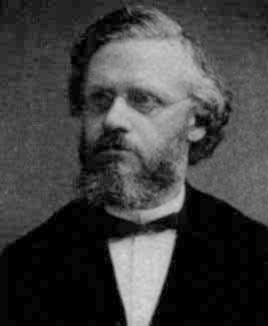
\includegraphics[width=.5\textwidth]{images/paul_bachmann}
\caption{German mathematician Paul Bachmann}

\pause 
% TikZ overlay for precise positioning
\begin{tikzpicture}[remember picture, overlay]
    \node[draw, fill=pink, rounded corners, cloud callout,  scale=0.7, font=\large, callout relative pointer={(0.5,-0.5)}] 
        at ([xshift=3.5cm,yshift=7cm]current page.south west) {Big O notation!};
\end{tikzpicture}
    
\end{figure}
\end{frame}





\begin{frame}
\small 
\begin{mygreenbox}[title=Definition]
Let $f$ and $g$ be real-valued non-negative functions defined on the same set of nonnegative integers. \\

Then $f$ is of order at most $g$, written \textbf{$\bm{f(n)}$ is $\bm{O(g(n))}$} ($f$ of $n$ is big-O of $g$ of $n$) if and only if there exist positive real number $B$ and integer $b$ such that
\[  |f(n)| \leq B |g(n)| \quad \text{for every integer } n \geq b\]	
\end{mygreenbox}
\vfill 
\begin{figure}
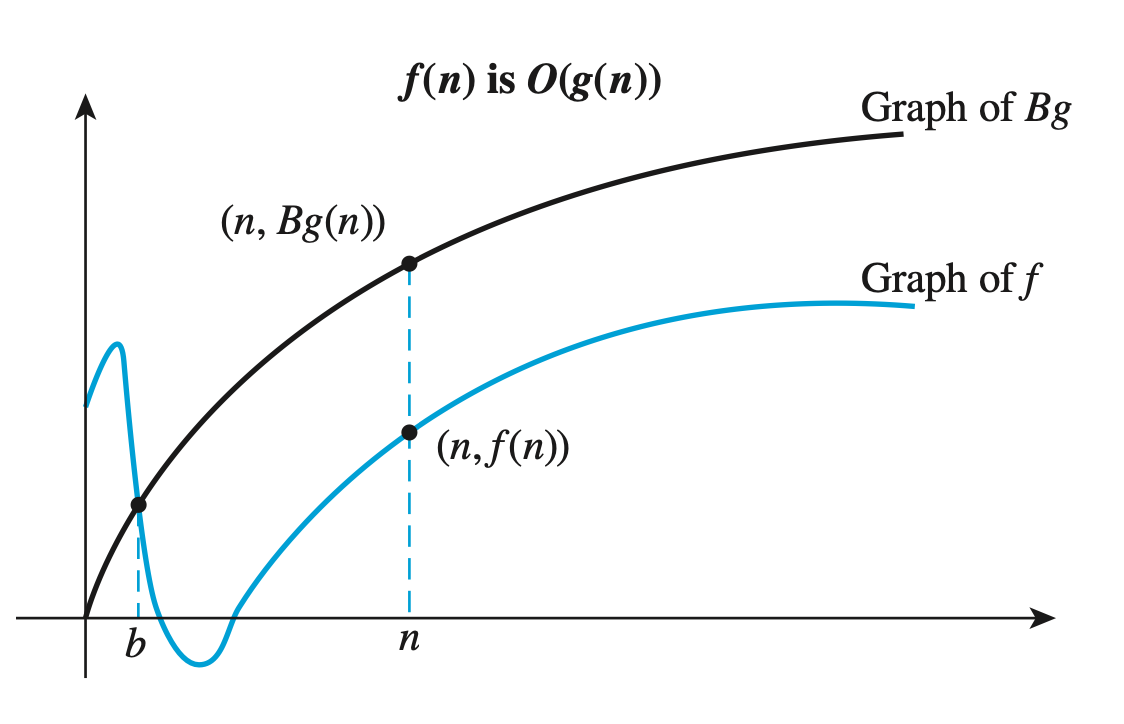
\includegraphics[width=.6\textwidth]{images/big_O.png}
\end{figure}
\pause \vfill 
\colorbox{yellow!30}{\textbf{Poll.}} How would you summarize this definition in words?
\end{frame}

\begin{frame}

\onslide+<1-> \colorbox{yellow!30}{\textbf{Poll.}} How would you summarize this definition in words?
\vfill 
\onslide+<2-> \colorbox{green!30}{\textbf{Solution.}}
The function $f$ is  \alert<4->{eventually} smaller in size than some \alert<4->{positive multiple} of $g$.  \\
\vfill 
\onslide+<3->  We say that \enquote{$f$ is of order at most $g$}.
\vfill 
%\onslide+<5->
%\colorbox{yellow!30}{\textbf{Poll.}} What's the deal with the highlighted words (especially \alert{positive multiple})?
\end{frame}


\begin{frame}{Classification Theorem}
\footnotesize 
\begin{center}
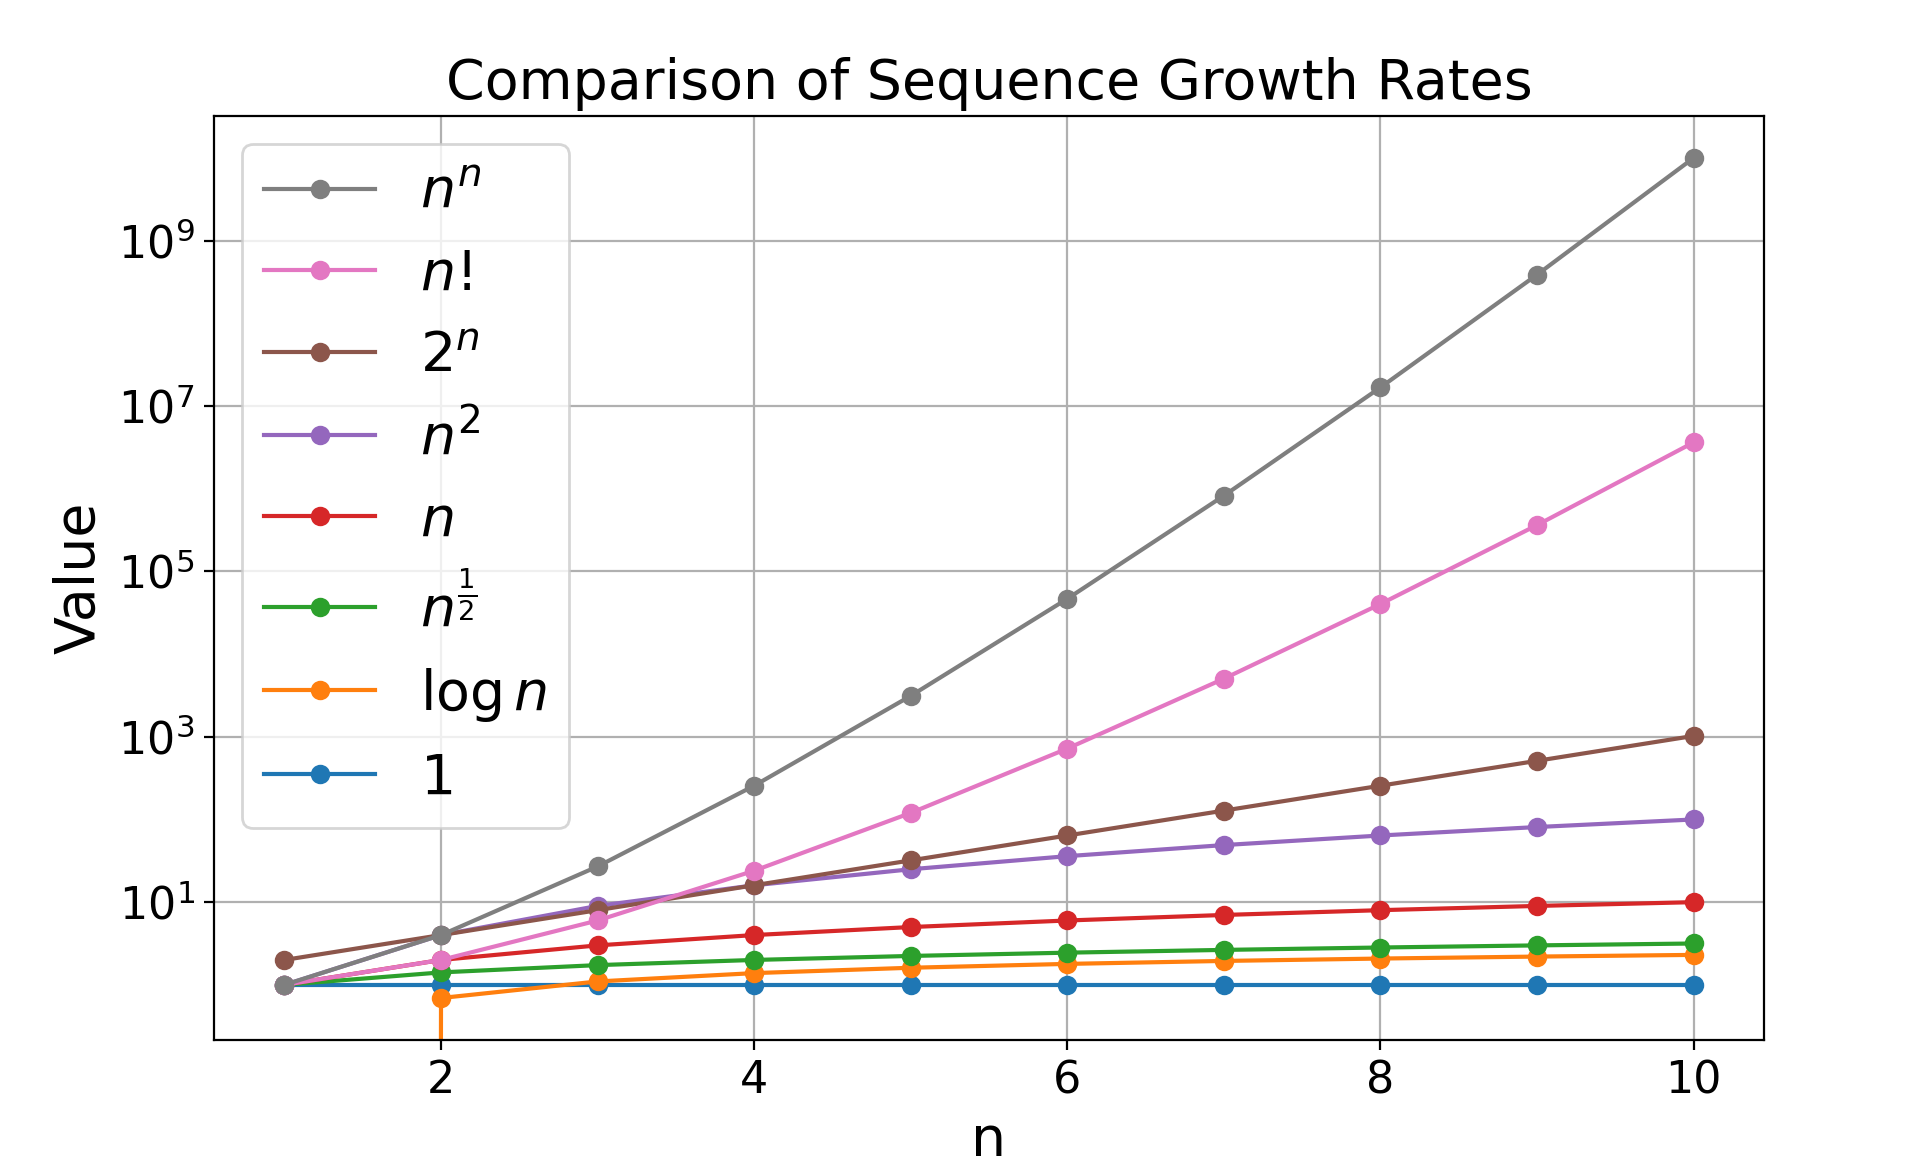
\includegraphics[width=0.7\textwidth]{images/classification_theorem.png}
\end{center}
\vfill 
\colorbox{yellow!30}{\textbf{Poll.}} How should we interpret this graph?
\vfill \pause 
\begin{itemize}
\item A taxonomy of growth rates (or scaling behavior): Any function is big O of everything equal to or above it, but is \textbf{not} big O of anything below it. \pause 
\item \textbf{Example}:  \colorbox{red!30}{$n$} is big O of \colorbox{red!30}{$n$}, \colorbox{purple!30}{$n^2$}, \colorbox{brown!30}{$2^n$}, \colorbox{pink!30}{$n!$}, and \colorbox{gray!30}{$n^n$}.  Even if we multiply  \colorbox{red!30}{$n$}  by a large constant, those functions will always eventually get bigger! \pause 
\item \textbf{Anti-Example}:  \colorbox{red!30}{$n$} is not big O of \colorbox{green!30}{$n^{\half}$}.  No matter how much you scale up \colorbox{green!30}{$n^{\half}$} by a large constant,  \colorbox{red!30}{$n$} will eventually get bigger!
\end{itemize}

\end{frame}





\begin{frame}{How to check Big O membership?}
\footnotesize 

\begin{mygreenbox}[title=\text{Example: $f(n) = 3n+100$ is $O(n)$}]
\textbf{Proof.} Take $n \geq 1$. Then 
\[ |3n+100| \leq  |3n+100n| = 103|n|.\]
\hfill (To satisfy the definition of big O, we take $b=1, B=103$.)
\end{mygreenbox}
\vspace{-.1cm}
\vfill 
\pause 
\begin{mygreenbox}[title=\text{Example: $f(n) = 9n^2+3n-2$ is $O(n^2)$.}]
\textbf{Proof.} Take $n \geq 1$. Then 
\[ |9n^2+3n-2| \leq  |9n^2+3n^2+2n^2| = 14|n^2|.\]
\hfill (To satisfy the definition of big O, we take $b=1, B=14$.)
\end{mygreenbox}
\small 
\vfill \pause 
\colorbox{red!30}{\textbf{Remark.}} Big O notation hides irrelevant details.
\vfill \pause 
\colorbox{yellow!30}{\textbf{Poll.}} Do you see a pattern?
\vfill \pause 
\colorbox{green!30}{\textbf{Solution.}} Polynomials are big O of their highest-order term.
\vfill \pause 
\colorbox{red!30}{\textbf{Remark.}} ...and also big O of still higher-order terms.   E.g. for $n \geq 1$,
\vspace{-.1cm}
\[14|n^2| \leq 14|n^3| \leq 14|n^4| \leq \hdots \]
\end{frame}



\begin{frame}{Classification Theorem: Zooming In On Polynomials}
\small 
\begin{center}
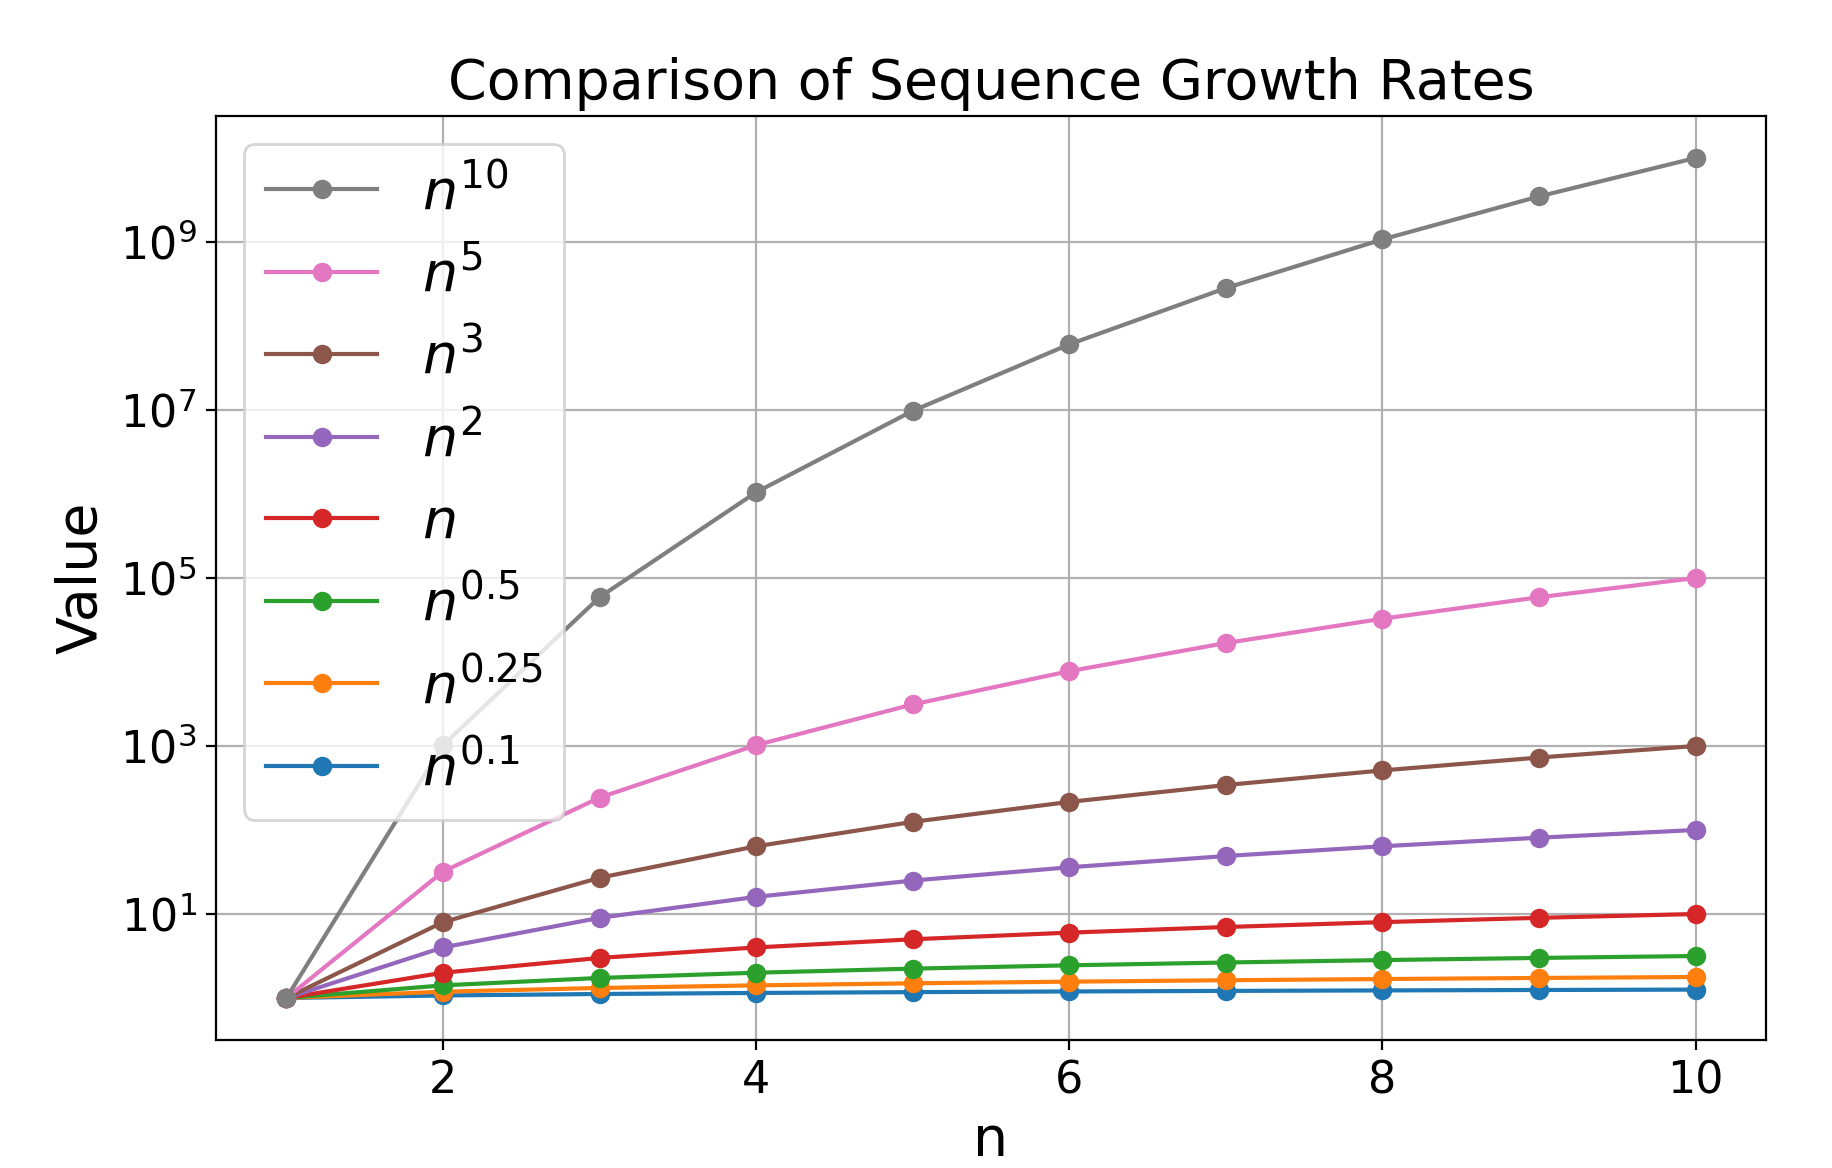
\includegraphics[width=0.65\textwidth]{images/big_O_polynomials.png}
\end{center}
\vfill 
\pause 
A taxonomy of growth rates: As you go down the legend, each function is big O of everything above it, but \textbf{not} big O of everything below it. \pause 
\vfill \pause 
\begin{myredbox}[title=Theorem]
For any function $f$ and positive real numbers $u$ and $v$ with $u<v$,
\[f \text{ is } O(x^u) \implies  f \text{ is } O(x^v)\]
\end{myredbox}

\end{frame}

\begin{frame}{A major problem with Big O statements}

\onslide+<1->
\colorbox{yellow!30}{\textbf{Poll.}} Suppose a person is analyzing the efficiency of algorithms, and finds that $f \text{ is } O(x^5)$ and $g \text{ is } O(x^4)$.  Because $4<5$, this person concludes that $g$ has a better algorithmic efficiency than $f$. Is this person's conclusion correct?
\vfill 

\onslide+<2->
\colorbox{green!30}{\textbf{Solution.}} No.  For instance, take $f(x) = x^2$ and $g(x)=x^3$. Then \\
\qquad \alert<3->{f}  \; is \; $O(x^2), O(x^3), O(x^4)$, \alert<3->{$O(x^5)$}, $\hdots$   \\ 
and  \\
\qquad \alert<3->{g}  \; is \;  $O(x^3)$, \alert<3->{$O(x^4)$}, $O(x^5)$, $\hdots$  \\
\vfill 
\onslide+<4->

\colorbox{red!30}{\textbf{Remark.}} The problem is that the upper bounds for Big O can be needlessly large! 

\vfill 
\onslide+<5->
 
We should interpret \enquote{$g \text{ is } O(x^4)$} as: \enquote{$g$ is of order \textbf{at most} $x^4$}.

\end{frame}


\begin{frame}{How to compare the efficiency of algorithms?}
\begin{figure}
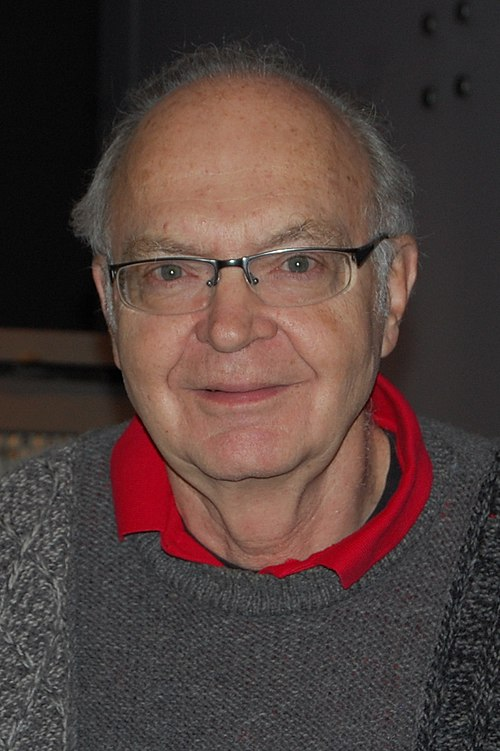
\includegraphics[width=.4\textwidth]{images/donald_knuth}
\caption{American computer scientist and mathematician Donald Knuth}

\pause 
% TikZ overlay for precise positioning
\begin{tikzpicture}[remember picture, overlay]
    \node[draw, fill=pink, rounded corners, cloud callout,  scale=0.7, font=\large, callout relative pointer={(0.5,-0.5)}] 
        at ([xshift=3.0cm,yshift=7.2cm]current page.south west) {Big Theta notation!};
\end{tikzpicture}
    
\end{figure}
\end{frame}

\begin{frame}{Overview: Big Theta combines Big O and Big Omega}
\small 

\begin{tabularx}{\textwidth}{c @{\hspace{0.25cm}} c @{\hspace{0.25cm}} c @{\hspace{0.25cm}} X}
\midrule 
\textbf{Big O} & $f \text{ is } O(g)$ & $f$ is of order \alert{at most} $g$  & The values of $f$ are  eventually \textbf{less} than those of a positive multiple of $g$. \\
 \vspace{.2cm}
\textbf{Big Omega} &  $f \text{ is } \Omega(g)$ & $f$ is of order \alert{at least} $g$  & The values of $f$ are  eventually \textbf{greater} than those of a positive multiple of $g$. \\
  \vspace{.2cm}
\textbf{Big Theta} &  $f \text{ is } \Theta(g)$ & $f$ is of order $g$ & The values of $f$ are  eventually \textbf{less} than those of a positive multiple of $g$ and  \textbf{greater} than those of a positive multiple of $g$.\\
\bottomrule
\end{tabularx}
	
\end{frame}

\begin{frame}
\begin{figure}
\includegraphics[width=\textwidth]{images/big_theta}
\end{figure}
\end{frame}


\begin{frame}{Big Omega: Definition}
\small 
\begin{mygreenbox}[title=Definition]
Let $f$ and $g$ be real-valued non-negative functions defined on the same set of nonnegative integers. 

\vfill 

Then $f$ is of order at least $g$, written \textbf{$\bm{f(n)}$ is $\bm{\Omega(g(n))}$} ($f$ of $n$ is big-Omega of $g$ of $n$) if and only if there exist positive real number $A$ and integer $a$ such that
\[  |f(n)| \geq A |g(n)| \quad \text{for every integer } n \geq a\]	
\end{mygreenbox}
\vfill 
\begin{figure}
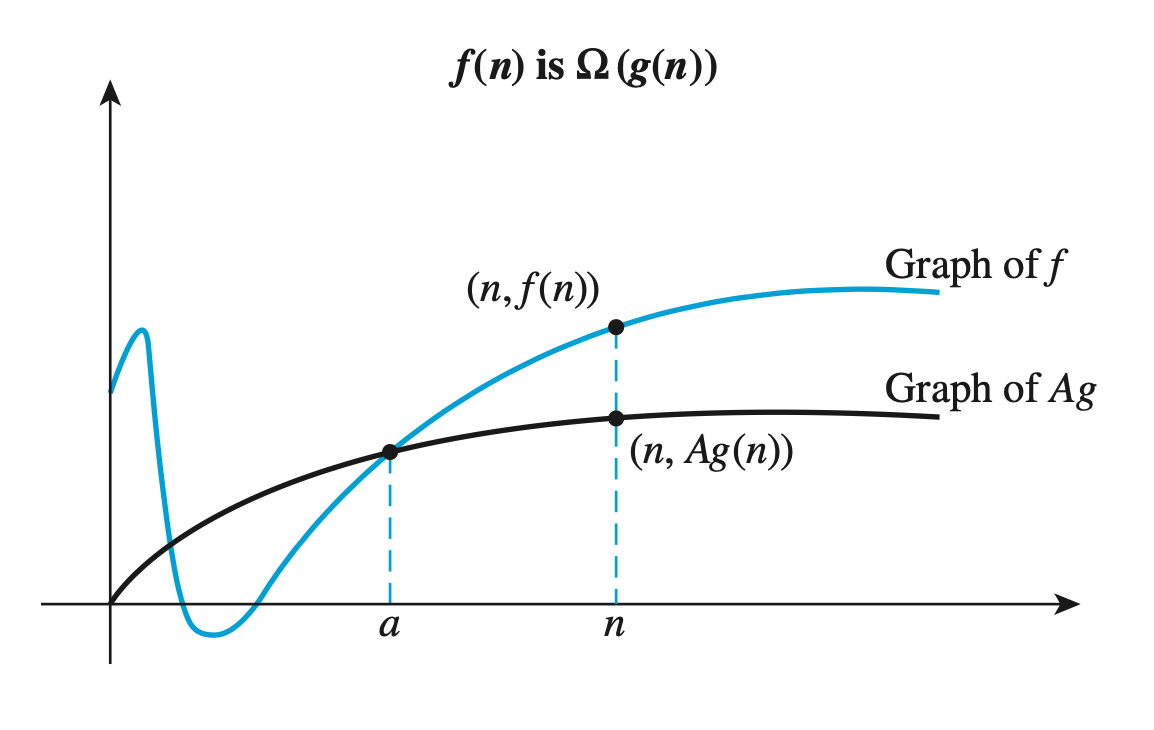
\includegraphics[width=.6\textwidth]{images/big_Omega.png}
\end{figure}
\end{frame}


\begin{frame}{Big Theta: Definition}

\begin{mygreenbox}[title=Definition]
Let $f$ and $g$ be real-valued non-negative functions defined on the same set of nonnegative integers. 
\vfill 
Then $f$ is of order $g$, written \textbf{$\bm{f(n)}$ is $\bm{\Theta(g(n))}$} ($f$ of $n$ is big-Theta of $g$ of $n$) if and only if $\bm{f(n)}$ is $\bm{O(g(n))}$ and $\bm{f(n)}$ is $\bm{\Omega(g(n))}$.
\end{mygreenbox}

\vfill 
\begin{figure}
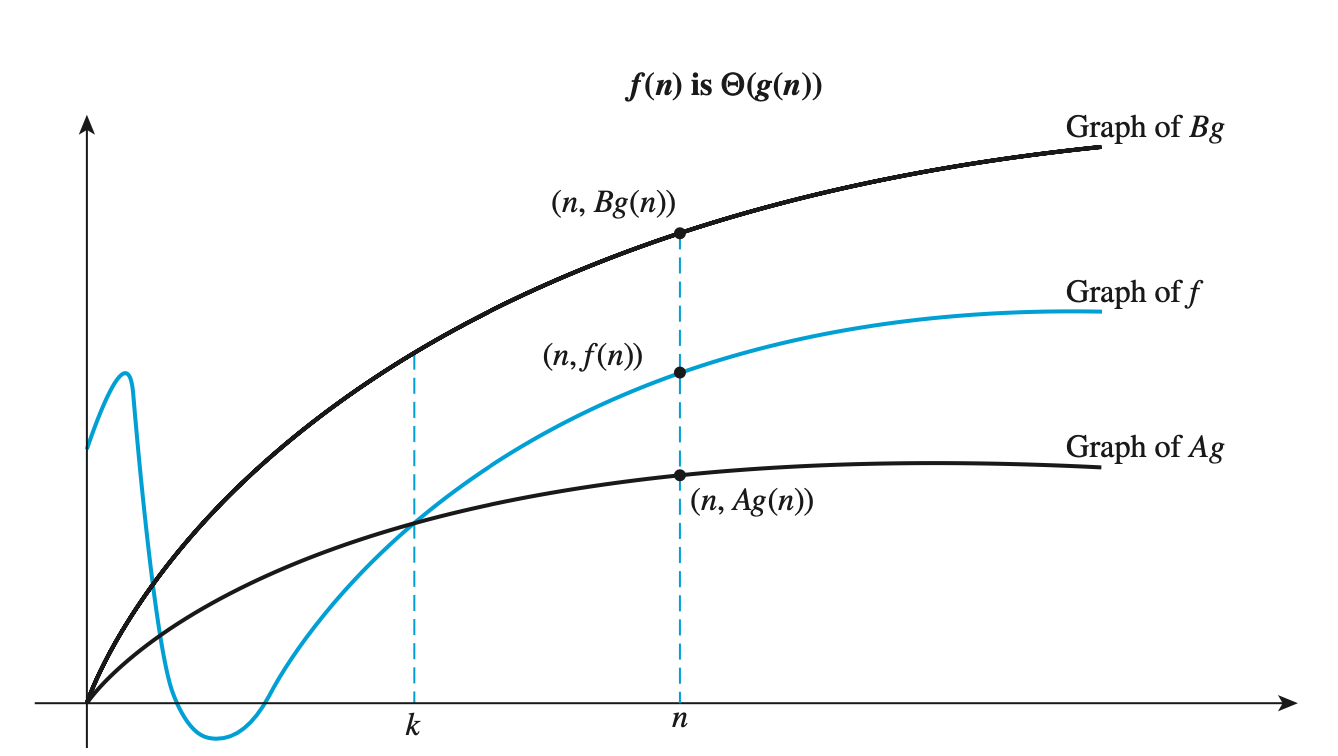
\includegraphics[width=.6\textwidth]{images/big_Theta_solo.png}
\end{figure}

\end{frame}




\begin{frame}{A useful theorem on Big Theta}

\begin{myredbox}[title=\text{Theorem: On Polynomial Orders}]
If $m$ is any integer with $m \geq 0$ and $c_0, c_1, c_2, \hdots c_m$ are real numbers with $c_m \geq 0$, then
\[c_m x^m + c_{m-1} x^{m-1} + \hdots + c_1 x + c_0 \text{ is } \Theta(x^m). \]
\end{myredbox}

\end{frame}






\begin{frame}[standout]
Group exercises
\end{frame}

\begin{frame}{Random group assignments}
\begin{columns}
\begin{column}{0.33\textwidth}
Ashley, Isabelle: 7 \\ 
Bailey, Tanna: 3 \\ 
Blaisdell, Olyver: 7 \\ 
Brown, Ashton: 10 \\ 
Cardenas, Dominic: 9 \\ 
Cutler, George: 12 \\ 
Fabik, Roland: 6 \\ 
Fellows, Audrey: 9 \\ 
Fitzgerald, Ryan: 11 \\ 
Fuller, Ryan: 3 \\ 
Griffen, Clara: 1 \\ 
Grutsch, Tanner: 2 \\\end{column}
\begin{column}{0.33\textwidth}
Hager, Nathan: 8 \\ 
Horner, Jayden: 10 \\ 
Johnson, Jaret: 5 \\ 
Kintzel, Samantha: 6 \\ 
Lameres, Alexis: 2 \\ 
Lee, Holden: 4 \\ 
Mayala, Reece: 1 \\ 
McLean, Connor: 5 \\ 
Mcbride, Daniel: 1 \\ 
Miller, Maverick: 9 \\ 
Moss, Emily: 8 \\ 
Mousseau, Matthew: 4 \\\end{column}
\begin{column}{0.33\textwidth}
Neuman, Evan: 4 \\ 
Putnam, John: 5 \\ 
Ramos, Vydel: 12 \\ 
Rathbun, Jedidiah: 6 \\ 
Roberts, Matthew: 11 \\ 
Roller, Nathan: 7 \\ 
Ryan, Otis: 8 \\ 
Shevtsov, Timothy: 2 \\ 
Stensland, Emma: 11 \\ 
Thiessen, Logan: 3 \\ 
Thompson, Jaiden: 12 \\ 
Vath, Ethan: 10 \\\end{column}
\end{columns}
\end{frame}

\begin{frame}{Group exercises}
\colorbox{green!30}{\textbf{Exercises.}}
\begin{enumerate}
	\item  Let $a_n = 1,000,000n + 3,000,000$. Prove that $a_n = O(n)$.
	\item Let $a_n = 5 + \frac{1}{n} + \frac{1}{n+1}$. Prove that $a_n = O(1)$.
	\item Let $a_n = n^2 + n + 1 + \frac{1}{n} + \sin n$. Prove that $a_n = O(n^2)$.
	\item Let $a_n = 3n^2 + 7$. Prove that $a_n = \Theta (n^2)$.
	\item Prove Theorem 7.9 from the Ponomarenko textbook. 
\end{enumerate}
\vfill
\colorbox{red!30}{\textbf{Note.}} Please solve all the problems above using the definitions of Big-O and Big-$\Theta$.
\vfill
\colorbox{blue!30}{\textbf{Theorem 7.9 (Ponomarenko).}} Let $a_n$ be a sequence, and $b_n,c_n$ be test sequences.  If $a_n = O(b_n)$ and $b_n = O(c_n)$, then $a_n = O(c_n)$.
\end{frame}


\begin{frame}{Solution to Group Exercise \#1}
\textbf{Problem.} Let $a_n = 1,000,000n + 3,000,000$. Prove that $a_n = O(n)$.
\vfill 
\textbf{Solution.}
%
For $n \geq 1$,
\begin{align*}
|1,000,000n + 3,000,000| \leq |1,000,000n + 3,000,000n| = 4,000,000 |n| 
\end{align*}
This satisfies the definition that  $a_n$ is $O(n)$ by setting $b=1$ and $B= 4,000,000$.

\vfill 
\textbf{Remark.} The notation ($b$ and $B$) comes from the definition of Big O given in this slide deck.
\end{frame}

\begin{frame}{Solution to Group Exercise \#2}
\textbf{Problem.} Let $a_n = 5 + \frac{1}{n} + \frac{1}{n+1}$. Prove that $a_n = O(1)$.

\vfill 
\textbf{Solution.}
%
For $n \geq 1$,
\begin{align*}
|5 + \frac{1}{n} + \frac{1}{n+1}| \leq |5 + 1 + 1| = 7 \cdot |1| 
\end{align*}
This satisfies the definition that  $a_n$ is $O(1)$ by setting $b=1$ and $B=7$. 

\vfill 
\textbf{Remark.} The notation ($b$ and $B$) comes from the definition of Big O given in this slide deck.

\end{frame}

\begin{frame}{Solution to Group Exercise \#3}
\textbf{Problem.} Let $a_n = n^2 + n + 1 + \frac{1}{n} + \sin n$. Prove that $a_n = O(n^2)$.

\vfill 
\textbf{Solution.}
%
For $n \geq 1$,
\begin{align*}
|n^2 + n + 1 + \frac{1}{n} + \sin n| &\leq |n^2 + n + 1 + 1 + 1| \\
& \leq |n^2 + n^2  + n^2  + n^2  + n^2 | \\
&= 5 |n^2|
\end{align*}
This satisfies the definition that  $a_n$ is $O(n^2)$ by setting $b=1$ and $B=5$. 
\vfill 
\textbf{Remark.} The notation ($b$ and $B$) comes from the definition of Big O given in this slide deck.

\end{frame}


\begin{frame}{Solution to Group Exercise \#4}
\textbf{Problem.} Let $a_n = 3n^2 + 7$. Prove that $a_n = \Theta (n^2)$.

\vfill 
\textbf{Solution.}
%
For $n \geq 1$,
\begin{align*}
|3n^2 + 7| &\leq |3n^2 + 7n^2| = 10 |n^2| 
\end{align*}
%
This satisfies the definition that  $a_n$ is $O(n^2)$ by setting $b=1$ and $B=10$.
\vfill 

Again for $n \geq 1$,
\begin{align*}
|3n^2 + 7| &\geq |3n^2| = 3 |n^2| 
\end{align*}
%
This satisfies the definition that  $a_n$ is $\Omega(n^2)$ by setting $a=1$ and $A=3$. 
\vfill 
Since $a_n$ is both $O(n^2)$ and $\Omega(n^2)$, we can conclude that $a_n$ is $\Theta(n^2)$.

\vfill 
\textbf{Remark.} The notation ($a,b,A,B$) comes from the definitions of Big O and Big Theta given in this slide deck.


\end{frame}


\begin{frame}{Solution to Group Exercise \#5}

\colorbox{yellow!30}{\textbf{Problem.}}  Prove Theorem 7.9 from the Ponomarenko textbook. 


\vfill
\colorbox{red!30}{\textbf{Theorem 7.9 (Ponomarenko).}} Let $a_n$ be a sequence, and $b_n,c_n$ be test sequences.  If $a_n = O(b_n)$ and $b_n = O(c_n)$, then $a_n = O(c_n)$.
\vfill 
\colorbox{green!30}{\textbf{Solution.}}
%
Since  $a_n = O(b_n)$, we have that for $n \geq b_1$,
\begin{align*}
|a_n| &\leq B_1 |b_n| \qquad \text{ for some constant } \; B_1.
\labelit \label{eqn:first_eqn}
\end{align*}
%
Since  $b_n = O(c_n)$, we have that for $n \geq b_2$,
\begin{align*}
|b_n| &\leq B_2 |c_n| \qquad \text{ for some constant } \; B_2.
\labelit \label{eqn:second_eqn}
\end{align*}
\vfill 
Hence for $n \geq \texttt{max} \set{b_1,b_2}$,
%
\begin{align*}
|a_n|  \stackexplain{\Eqref{eqn:first_eqn}}{\leq} B_1 |b_n| \stackexplain{\Eqref{eqn:second_eqn}}{\leq} B_1 \cdot B_2 |c_n| 
\end{align*}
%
This satisfies the definition that  $a_n$ is $O(c_n)$ by setting $b=\texttt{max} \set{b_1,b_2}$ and $B=B_1 \cdot B_2$. 
\end{frame}

\end{document}
